\documentclass{llncs}

\usepackage{listings}
\usepackage{csquotes}
\usepackage{color}
\usepackage{caption}
\usepackage{graphicx}
\usepackage{zed}
\DeclareGraphicsExtensions{.pdf,.png,.jpg}
 \usepackage{listings}
 \usepackage{courier}
 \lstset{
         basicstyle=\footnotesize\ttfamily, % Standardschrift
         %numbers=left,               % Ort der Zeilennummern
         numberstyle=\tiny,          % Stil der Zeilennummern
         %stepnumber=2,               % Abstand zwischen den Zeilennummern
         numbersep=5pt,              % Abstand der Nummern zum Text
         tabsize=2,                  % Groesse von Tabs
         extendedchars=true,         %
         breaklines=true,            % Zeilen werden Umgebrochen
         keywordstyle=\color{red},
    		frame=b,         
 %        keywordstyle=[1]\textbf,    % Stil der Keywords
 %        keywordstyle=[2]\textbf,    %
 %        keywordstyle=[3]\textbf,    %
 %        keywordstyle=[4]\textbf,   \sqrt{\sqrt{}} %
         stringstyle=\color{white}\ttfamily, % Farbe der String
         showspaces=false,           % Leerzeichen anzeigen ?
         showtabs=false,             % Tabs anzeigen ?
         xleftmargin=17pt,
         framexleftmargin=17pt,
         framexrightmargin=5pt,
         framexbottommargin=4pt,
         %backgroundcolor=\color{lightgray},
         showstringspaces=false      % Leerzeichen in Strings anzeigen ?        
 }
 \lstloadlanguages{
         Java
 }
%\DeclareCaptionFont{blue}{\color{blue}} 

 %\captionsetup[lstlisting]{singlelinecheck=false, labelfont={blue}, textfont={blue}}
 % \usepackage{caption}
 
\DeclareCaptionFont{white}{\color{white}}
\DeclareCaptionFormat{listing}{\colorbox[cmyk]{0.43, 0.35, 0.35,0.01}{\parbox{\textwidth}{\hspace{15pt}#1#2#3}}}
 % \captionsetup[lstlisting]{format=listing,labelfont=white,textfont=white, singlelinecheck=false, margin=0pt, font={bf,footnotesize}}
 
    \graphicspath{{figs/}}
 


\captionsetup[lstlisting]{format=listing,labelfont=white,textfont=white, singlelinecheck=false, margin=0pt, font={bf,footnotesize}}




% we define a set of macros for constants of type 'Kind' 

\def\datamodel{\mathsf{datamodel}}
\def\dataclass{\mathsf{dataclass}}
\def\dataelement{\mathsf{dataelement}}
\def\enum{\mathsf{enum}}
\def\enumeration{\mathsf{enumeration}}
\def\primitivetype{\mathsf{primitivetype}}
\def\datatype{\mathsf{datatype}}

% and for multiplicity 

\def\optional{0{\upto}1}
\def\mandatory{1{\upto} 1}
\def\many{0{\upto}*}

% our partial ordering on constraints

\def\Cimplies{\mathrel{\implies_c}}
\def\Ciff{\mathrel{\iff_c}}

% our partial ordering on text (this will become interesting later)

\def\Timplies{\mathrel{\implies_t}}
\def\Tiff{\mathrel{\iff_t}}

% and conjunction 

\def\Tand{\mathrel{\land_t}}
\def\TAnd{\mathop{\land_t}}

% our globalised version of the defining relations

\def\refines{\mathrel{refines}}
\def\newVersionOf{\mathrel{newVersionOf}}
\def\extends{\mathrel{extends}}
\def\contains{\mathrel{contains}}

% we may have \sqsubseteq and \gg when it comes to analysis 

% our two status values 

\def\draft{\mathsf{draft}}
\def\final{\mathsf{final}}

\usepackage{zed}

\begin{document}

\title{Metadata Registry and management based on ISO11179 using Model Based Engineering}
%If Title is too long, use \titlerunning
%\titlerunning{Short Title}

%Single institute
\author{Jim Davies, David Milward \and Seyyed Shah}
%If there are too many authors, use \authorrunning
%\authorrunning{First Author et al.}
\institute{University of Oxford}
\maketitle

\begin{abstract}
In this paper we present an ISO11179 metadata registry using a data-oriented Domain Specific Modelling Language (DSML). In particular we examine how certain aspects of the ISO11179 specification can be strengthened by using a specific DSML built to handle interoperability use cases, and also how using a model based engineering framework addresses ambiguities in the standard. We examine how the DSML approach taken in this paper presents a concrete realisation of data componentisation, harmonisation, standardisation and reuse of meta-data components. We also examine how the ISO11179 based DSML can be implemented using the Eclipse Modelling Framework and made interoperable with UML In particular, we identify how Model Driven Engineering has helped in achieving the specific goals of ISO11179 via a case study.

\end{abstract}

\keywords{...}

\noindent

\section{Introduction}

This paper describes the process of defining a metalanguage for use in a metadata registry using Model Based Engineering.  Initially the requirement came from the requirement for researchers to curate datasets for clinical usage. Previous work on implementing metadata registries conforming to ISO11179 informed this exercise, so whilst the core requirement came from users, an attempt was made to adher to ISO11179 in the process in the hope of making the metadata registry interoperable with other ISO11179 comformant registries. To achieve this we address several challenges including the formalisation of an ISO standard in Z and the creation of an intermediate model-driven formalism to support the creation of a practical result: a tangible applications for metadata management.

ISO11179 is an internationally recognised standard for metadata registries. Metadata registries are used within organisations to ensure critical data is used consistently. In recent times, the amount and complexity of data available to organizations has exploded and standards such as ISO11179 have become essential. Yet, there are several functional areas of the standard that are ambiguous and open to interpretation and the standard only partly formalises metadata management processes. `High-level' processes of a registry are described, but defined in natural language, so have been implemented in a variety of ways. For example the standard discusses publication and versioning of metadata and states that models must not be edited after publication but does not specify what this means can be achieved in practice. %(Seyyed: @David could you check this last claim is correct?)

A lack of semantics in the standard becomes a greater issue when there is more than one implementation of the standard or implementations are expected to interoperate with external systems. There are several examples of tools that claim ISO11179 conformance and despite the existence of an international standard, each makes varying assumptions and opaque interpretations of that standard. A possible solution to this problem is to define an clear and unambiguous interpretation of standard, and use this as a basis to derive an implementation. Although the structural elements of the standard may be interpreted relatively straightforwardly using UML, and such as the approach has already been taken in the CaBIG~\cite{Kunz2009} initiative, the functional aspects of the standard remain open.

To resolve this mismatch, we propose a formal approach to reasoning about the standard and a practical approach to implementation. The Z notation supports unambiguous reasoning about human written specifications  and is based on based on classical Z-F set theory. A number books and papers describing the notation and applications are available~\cite{woo96}. At the heart of Z is first order predicate logic with quantification. Users can formally verify properties in a specification, and has been used in numerous examples (\cite{woo96}). Although Z is often dismissed for lacking tool support and having a steep learning curve for the average programmer, it is useful in this context. The major advantage to Z is the specification need only be formalised once by experts and implementations can be derived from that formal specification.

The aim of Model Driven Engineering (MDE) is describing key abstractions of a system, and using those to derive implementations. This makes MDE an appealing basis to build a metadata registry. Model driven engineering techniques can be used to define languages and semantic mappings pairs of languages, for example between specification and design languages or design and implementation languages. However, we diverge slightly from this approach towards a higher level of abstraction: metamodelling. We use a detailed language in Z to derive a metamodel for metadata, which forms a Domain Specific Modelling Language (DSML). The models created by users in this DSML represent the metadata in a particular context and organisation. 

This paper applies international standards, formal methods and model driven development to build a reasoned metadata registry. This tool is tested within a number of projects in the clinical and healthcare domains, within the UK National Health Service (NHS). We have examined the strengths and weaknesses of the approach taken and the ISO11179 standard, and present the results of our research in this paper. 


\section{Backgound}

\subsection{Model Based Engineering}
Model Based Engineering or Model Driven Engineering is the software engineering practise which utilises \emph{Models} as first class entities in analysing and designing software artefacts; code is generated directly from the models, updates are made directly to the models and the code is then regenerated. A situation is achieved whereby a complete round-trip is possible from the model to the code, and then from the code back to exactly the same model. Full round tripping is not always achieved in practise, and sometimes the modelling simply serves as an initial design, from which a shell is generated and the code is completed by software developers. However considerable gains in code generation and prototyping can be achieved, and these make the modelling process worthwhile.

In MBE the overall architecture of a software project is often classified using the notion of abstraction layers. Abstraction is used in many design processes, in software engineering many sub-processes lend themselves to various kinds of mathematical modelling.  In object oriented design objects are used as the main components of a program, rather than sub-routines or functions.  These objects can be \emph{abstracted} to a kind of templated object called a \emph{class}, a class will contain a blueprint for both data and methods.  Using this idea we consider the the program running, that is the interaction of different objects, to be at level M0.  At this level the program will consist of different objects interacting according original program code, which is written for the most part a collection of various \emph{classes}.  The program code, in effect the blueprint for the program, is considered to be an abstraction of the running program, and is considered to be at level M1.  A model or program at level M1 is defined by a blueprint of model, in effect a \textbf{meta-model} which exists that level M2, and likewise a \textbf{meta-model} can be defined at a higher level of abstraction.  This abstraction \emph{layering} can continue ad-infinitum, however most MBE practitioners use 4 levels, indeed the Model Driven Architecture agreed and specified by the OMG \cite{MOF242}, also known as the Meta Object Facility (MOF) currently limits itself to 4 layers, which are illustrated in Figure~\ref{fig:mbe1}

\begin{figure}[h]
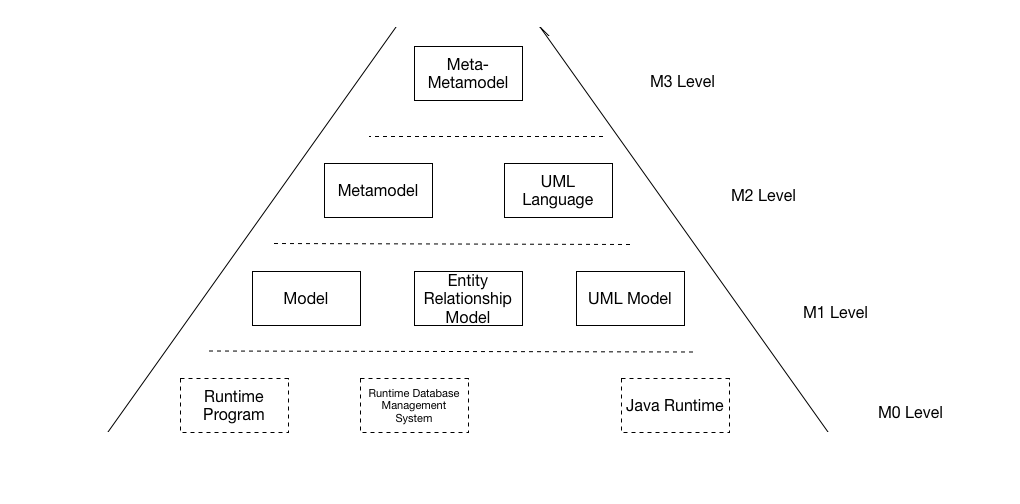
\includegraphics[width=1.0\textwidth,natwidth=610,natheight=642]{Models1}
\caption{Abstraction Layers in Model Based Engineering} 
\label{fig:mbe1}
\end{figure}

We can see that UML itself sits at what is refered to as the M2 level in this architecture model. Each abstraction layer is defined so that the level \emph{below} can be seen as being an implementation of that layer; in this way the UML model is one implementation out of many possible implementations of the UML language. The UML Language itself is an implementation of the MOF meta-meta-language which resides at the M3 layer. It is possible to use UML to define other meta-models at the M2 level, one could for instance use a sub-set of UML to define just a data language at this level.

When one builds a model for a system using MBE the model is at the same level of abstraction as the program, and can be seen as different way of representing the same thing.  A Java or C\# program therefore would sit at the M1 level, and would have a direct one-to-one relationship with a UML model at that level. The idea being that by building the model in say UML one can automatically generate the code in java.

\subsubsection{Domain Specific Languages(DSL)}
The term \emph{Domain Specific Language} is used to talk about a language which has been built purely to be used within one narrow domain of concern. It is more specialized than a general purpose language, but will generally make writting program code within that narrow domain easier.  An example here would be the language \emph{Gradle} which has been built to solve the problem of managing software development projects, and uses as first class citizens the nouns and verbs of the software development process, such as \emph{clean, run, process, etc}. It allows a domain expert to write a build process from scratch without having to know how to do a lot of the detailed work in the programming language. Gradle is written in Groovy, and compiles to the JVM, however it used by software developers developing in both JVM and non-JVM languages alike.

The term DSL is a general term and covers many different types of language.  For our purposes here we consider two main aspects of software analysis and design, the first is the modelling of the domain and the second is engineering an efficient programming language to express these models.These two aspects are often merged, however the two aspects are sometimes treated separately as with the layered modelling approach taken by Latry et al~\cite{latry2006processing}. 


\subsubsection{Domain Specific Modelling and Programming Languages}

A Domain Specific Modelling Language (DSML) is one that is purely targeting the problem domain, in that it describes problems and solutions in domain terms, and provides a language which domain experts can understand and implement within their domain. In this regard we are considering the domain of managing large datasets, ontologies and classification systems, and the domain experts we are considering are those who will create and edit these datasets. A Domain Specific Programming language(DSPL) is concerned with how to implement a suitable language using a general purpose programming language(GPL), frameworks, aspects, etc. There are no real rules to developing a DSPL, and it maybe that developing a DSPL is simply a stage in the development of the DSL, or it may be a module within the DSL. For the most part we haven't defined a DSPL for this project, the implementation has been carried out using the Groovy language, or with the XTend/Java toolkit in Eclipse. 

\subsubsection{Platform Independent and Specific Implementation}
In the Model Driven Architecture (MDA)~\cite{frankel2003model} of the OMG models are viewed as being either \textbf{Platform Independent Models(PIM)} or \textbf{Platform Specific Models (PSM)}, a division which is similar in concept, but not identical to the DSML/DSPL split previously described. The idea is that a PIM should model the problem and be independent of any computer operational issues, in this way a model in one language can be transformed to another language without any reference being made to platform-specific concerns such as memory usage, persistance constraints, big-endianness etc.


\subsection{ISO11179}

The ISO11179 Standard for metadata registries defines its purposes (ISO11179-1 section 0.2 General description of ISO/IEC 11179)as follows,
\newline
to promote:
\begin{itemize}
\item Standard description of data
\item Common understanding of data across organizational elements and between organizations
\item Re-use and standardization of data over time, space, and applications
\item Harmonization and standardization of data within an organization and across organizations
\item Management of the components \emph{of descriptions} of data
\item Re-use of the components \emph{of descriptions} of data.
\end{itemize}
ISO/IEC 11179 is in effect a standard for metadata-driven exchange of data in an heterogeneous environment, based on exact definitions of data. Interoperability isn't explicitly mentioned as aan aim, however these six aims/purposes are very close to being a description of a framework for interoperability for data and data components through the use of \emph{metadata}. There is no international standard which specifically addresses interoperability, although there are a number of accepted maturity models which address interoperability issues(NIEM, ECInterop) within the enterprise.  %%The MDI model framework which emerged from the Athena and Interop NoE (INTEROP, Athena) research projects have made progress in defining ways of implementing interoperability using model driven engineering concepts and ideas, and since ISO11179 is currently in use in both the Healthcare and Defence sectors we examine the core purposes of the standard to try and determine how we it achieves these purposes. %%
The standard itself is not a specification for building a physical or logical metadata registry, but rather a set of semantic principles on how data relationships should be handled. We implement an ISO11179 conformant metadata registry using Model Based Engineering principles, and examine how use of these principles have helped achieved the purposes of ISO11179. The biggest problem we had with the design of a metadata registry based on the ISO11179 standard was in interpreting the requirements in a way that ensured that we ended up with useful toolkit for handling metadata, much of which was specified using XML Schema, relational database schemas or very often in excel spreadsheets. The ISO11179 gives a robust treatment of the semantic aspects of metadata, and even provides illustrations of many aspects of the standard using UML 2.4.1, however translating that into a model based design was difficult for several reasons. Firstly the standard uses text and UML to provide a description, indicating that text takes precedance over UML where there is an ambiguity, or chance of mis-interpretation. Secondly the standard doesn't really discriminate between the model for metadata and the model for the registry itself, and while the two are closely related it is sometimes difficult to know whether the standard is refering to the metadata or the registry. For these reasons it was decided to translate the specification in the standard into a formal specification language in order to have a unambiguous basis on which to build a model for the registry. We used the Z specification language, it is a specification language based on set theory and first order logic and has been used to specify the W3C's Web Services Description Language~\cite{WSDL}.

\subsection{Z Specification Language}

The Z notation is a specification language built on first order logic and set theory. Z works with sets of objects that are classified by type, using both propositional and predicate logic. By using Z one is able to analyse both domain objects and computational constructs by linking the textual description and syntax to a formally defined semantics. 
\subsubsection{Sets}
Sets can be defined, and thus introduced into a specification, using a simple declaration. Sets can be defined and reasoned about by forming statements using propositional and predicate logic. Using standard propositional operators, such as `is element of', `is not an element of', `not', `or','and', `implies','if and only if','union','intersection': \begin{zed}\in, \notin, \lnot, \lor,\land, \implies, \iff, \cup, \cap,  \end{zed}\\ the Z specification language allows unambiguous statements and propositions to be made, and thus reasoning can be carried out on such a formal specification. This is extended to include first order logic with the use of quantifiers, which allow a single entity, or all entities to be identified, as follows: \begin{zed}  \exists y:Y | A \spot B \\ \forall x:X | P \spot Q   \end{zed}
\subsubsection{Types}
If we introduce a variable in Z we need to declare it's type. Everything introduced in Z needs to have a type and that type needs to be defined, each variable or expression can belong to only one type.
\subsubsection{Definitions}
The simplest definition which declares a variable and makes a statement about it in the form of a predicate is called an \emph{axiomatic definition}, and it takes the form:
	\begin{axdef}
	Declaration
	\where
	Predicate
	\end{axdef}
Generic definitions are introduced as follows:
\begin{gendef}[Params]
	Declaration
	\where
	Predicate
\end{gendef}
\subsubsection{Relations}
Z contains the constructs to deal with relations, normally by using the idea of \emph{domain} and \emph{range}. We can use this to make statements about people and things using relationships and relationship operators. 
\begin{zed}
drives = {George \mapsto renault}
\end{zed} simply states that George drives a renault. We can assume therefore that George is in the \emph{domain} of the set of people that are driving cars, and that renault is in the set of cars that are driven. The Z notation allows us to specify \emph{functions} and to differentiate between types of functions: partial, total, bijections Z has a number of other operators which can be used to specify items included in a range or domain, so that quite complex rules can be declared for sets of variables. By using the various relational operators in Z we can arrive at a map of how relationships exist within a domain.
\subsubsection{Schemas}
The basic unit of specification in Z is not the set decalaration, but the \emph{schema} which allows variables to be introduces together with rules and predicates governing their structure and behaviour. The schema is used to structure and compose descriptions, allowing renaming and thus re-use, and most importantly allowing concerns to be grouped together thus making the mathematical formulation easier to read and reason with. It differs from an axiomatic definiton in that it has a name, and thus can be used as a component in another schema, which is a feature that enables composition and decomposition of components within the specification.  
To illustrate this we declare sets of Identifiers (ID) and dataitems (DI):
\begin{zed}
 [ID, DI]
 \end{zed}
\begin{schema}{MetadataRegistry}
 dataItems: \power DI\\
 registry: ID \fun DI\\
 \where
 dataItems = \ran registry
\end{schema}
This schema is a formal description of a metadata registry which contains a set of dataItems which are linked to identities, the schema introduces the set of DataItems, and the registry as functional relationship between identities and dataitems such that the domain can be defined by the set of identities and the range can be defined by the set of dataitems. Clearly more variables, sets and constraints can be introduced, and indeed will be when we come to specify the metadata registry, however this demonstrates the way in which Z specifications are composed.
\subsubsection{Object Z}
Object Z is an extension to the Z notation which allows classes to be specified in what amounts to an extended schema. It is a useful extension for specifying object oriented constructs, although most specifications can be completed using the standard Z notation. We will introduce constructs as necessary during the course of the Z analysis. 


\section{Design of an ISO11179 Metadata Registry}

The ISO11179 standard as discussed describes a metamodel using text and UML 2.4. In order to arrive at a working model based specification we have taken that description and written it using a formal specification language.  This enabled us to generate both the registry and some of the transformations required to express datasets in terms of the standard.  ISO11179-3 has a detailed account of the registry metamodel and its attributes, and sets out to be relevent to application designers, system architects, and software developers. It uses UML 2.4.1 as a modelling language to describe the main features of a conformant metadata registry, although the standard itself is quite clear in not endorsing any particular environment, database management system, database design paradigm, system development methodology, data definition language, command language, system interface, user interface, computing platform or technology required for implementation. However in ISO11179-3.5 a metamodel is used to describe the information model of a metadata registry, and again the standard is clear that this should not limit the actual implementation technology used. The UML description is split into a number of packages:
\begin{itemize}
\item Basic Package
\item Identification Metamodel
\item Designation and Definition Metamodel
\item Registration Package
\item Concepts Package (Concepts and Classification regions)
\item Binary Relations Package
\item Data Descriptions Package
\end{itemize}

The standard continues to provide a detailed account of how metadata items are related within the metadata registry, for the purposes of brevity we will not repeat them all here, but we may refer back to specific parts of the standard where required.

This section details a brief account of the specification of the ISO11179 registry which was carried out using Z. From the resulting Z specification we have built the DSML on which we have built the metadata registry. The metadata registry has then been used for the creation, curation and management of a variety of datasets which we detail in the Results section. 

The metamodel or language for data we describe is informed by our experience with Healthcare information systems which is documented in a previous paper \cite{DSMCR} and by the development of an open source Metadata Registry built around similar principles. The DSML has been built to help with data curation and creation in the Healthcare domain, and as such is the result of discussion with domain experts in this sector. The reason for designing this DSML is that we seek a meta-language to be able handle hetrogeneous metadata stored using a variety of languages. It needs to be able to capture metadata, in particular a detailed description the data is stored in relational databases, XML Schemas, XML files based on XML Schemas, Excel files and object-oriented programs. It then needs to be able to automatically transform the data into a number of simple formats. To do this each dataset at an M1 level needs to be described at the M2 level, by doing this we can build a container which can hold the metadata collected at the M1 level.

The metamodel in ISO11179-3 is defined in terms of UML and text, and the description is split into a number of packages, which we review in brief.
\begin{zed}
[Packages,basicPackage, IdentificationMetamodel, \\
DesignationAndDefinitionMetamodel,RegistrationPackage, \\
ConceptsPackage, BinaryRelationsPackage, DataDescriptionsPackage]

\end{zed}

ISO11179-3sect1 describes the scope of the documents, and states that sections 5-11 form a specification of a \emph{Platform Independent Model} for a metadata registry. Section 12 describes basic attributes for metadata items in a situation where a full metadata registry implementation is not available or possible. Section 2 deals with normative references, the only indispensible referenced document listed is ISO11179-6. Section 3 introduces terms, we will make reference to this section where needed in the course of this specification.Section 4 deals with conformance and is not directly relevent to the work here.

We start with section 5 which details the overview of the packages involved with the MDR, indeed it is described as a metamodel for the infomraiton model of a MDR. This metamodel is terms the \emph{Registry Metamodel} and is specified as a \emph{conceptual data model - one that describes how relevant information is structured in the natural world, in other words how the human mind is accustomed to thinking of the information}. It must be observed that the previous statement is factually incorrect and demonstrates the enormous arrogance of the ISO11179 committee members, who demonstrate very little understanding of current neuro-science, especially recent insights into how the human mind is or is not accustomed to handling information, the only reason to continue with this twaddle is to demonstrate once and for all what an inadequate document it is.

Section 5 continues by stating that there is no one-to-one match between attributes of the metamodel and fields, columns or other database artefacts, and it emphasises the fact that the physical implementation may or may not be distributes, implemented using databases, XML, RDF/OWL or any other related information processing systems. However it does go on to state that minimum and maximum constraints of attributes should be enforced at all times, and that constraints on minimum occurences are to be enforced when the registration status of the metadata item is "recorded" or higher. It would seem that the latter statement is overruled by the former statement, so it is ignored for this specification.

The standard uses the term \emph{metamodel construct} to refer to the UML model constructs or artefacts being used, and \emph{metadata object} for the model being specified, UML 2.4.1 is used in the version being examined. The metamodel is split into six packages and the dependencies between them are illustrated in Figue ~\ref{fig:pack}, some are further subdivided into "regions" (although this is not a formal UML term).

\begin{figure}[h]
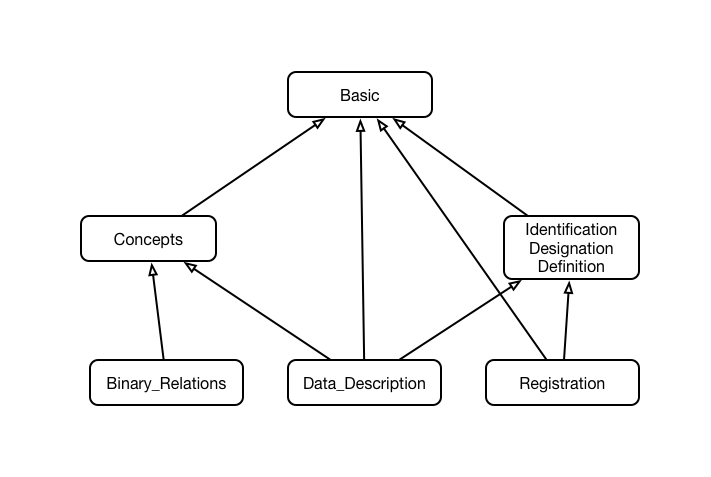
\includegraphics[width=1.0\textwidth,natwidth=610,natheight=642]{ISOPack}
\caption{Data Description Model} 
\label{fig:pack}
\end{figure}

There are 3 types of dependency listed : subclassing between packages, relationships and referenced datatypes.

A metadata item may be "extended by" any one of six related stereotypes, based on classes which are covered in later sections, they are \emph{Identified\_Item}, \emph{Registered\_Item},\emph{Administered\_Item},\emph{Attached\_Item},\emph{Designatable\_Item},\emph{Classifiable\_Item}.
\begin{zed}
[Scoped\_Identifier,metadataItem,Designation,Definition,Concept,Submisson\_Record,\\
Stewardship\_Record,Registration\_Authority,Administered\_Record]
\end{zed}

\begin{schema}{IdentifiedMetaDataItem}
identification\_association: metadataItem \pfun Scoped\_Identifier \\
\where
 \#identification\_association \leq 1 \\
\end{schema}

\begin{schema}{DesignatedMetaDataItem}
item\_designation\_association: metadataItem \pfun Designation \\
\where
 \#item\_designation\_association \leq 1 \\
\end{schema}

\begin{schema}{DefinedMetaDataItem}
item\_definition\_association: metadataItem \pfun Definition \\
\where
 \#item\_definition\_association \leq 1 \\
\end{schema}

\begin{schema}{ConceptMetaDataItem}
classification\_association: metadataItem \pfun Concept \\
\where
 \#classification\_association \leq 1 \\
\end{schema}

\begin{schema}{RegisteredMetaDataItem}
identification\_association : metadataItem \pfun Scoped\_Identifier \\
submission\_association : metadataItem \pfun Submisson\_Record \\
\where
 \#identification\_association \leq 1 \\
 \#submission\_association \leq 1 \\
\end{schema}

\begin{schema}{AdministeredMetaDataItem}
identification\_association: metadataItem \pfun Scoped\_Identifier \\
submission\_association: metadataItem \pfun Submisson\_Record \\
stewardship\_association: metadataItem \pfun Stewardship\_Record \\
registration\_association: metadataItem \pfun Registration\_Authority \\
attachment\_association: metadataItem \pfun Administered\_Record \\
\where
 \#stewardship\_association\leq 1 \\
 \#registration\_association \leq 1 \\
 \#attachment\_association = 0 \\
 \#identification\_association \leq 1 \\
\end{schema}

\begin{schema}{AttachedMetaDataItem}
stewardship\_association: metadataItem \pfun Stewardship\_Record \\
attachment\_associations: metadataItem \pfun Administered\_Record \\
\where
 \#attachment\_associations \leq 1 \\
 \#stewardship\_association = 0 \\
\end{schema}


A metadataItem may be extended with \emph{Slots} which allow the metadataItems to be extended with custom attributes, relationships, classes and even complete new packages.
\begin{zed}
[String]
\end{zed}
\begin{schema}{Slot}
  key: \nat \\
  value: String \\
\end{schema}

\begin{schema}{ExtendedMetaDataItem}
	slot\_association: metadataItem \pfun Slot \\
\where
 	\#slot\_association \geq 0 \\
\end{schema}

  

\subsection{ISO11179:3 Basic Package}

This section introduces a number of basic types, some of which are already defined in Z (Boolean, Integer and Natural Range - or Natural Number), the others we can introduce as follows:
\begin{zed}
[ Date, Value, Sign, PostalAddress, Datetime,  Text,Notation, PhoneNumber]
\end{zed}
This section introduces the basic types, together with a number of classes: ReferenceDocument, DocumentType, Contact RegistrationAuthorityIdentifier, Individual, LanguageIdentification, Role, Organization.


subsubsection{Classes overview}


\begin{class}{Reference\_Document}
\also
identifier : String \\
document\_type : Document\_Type \\
language : Language\_Identification \\
notation: Notation \\
title : Text\\
provider: Organization\\
url: Strin
\end{class}




\subsection{ISO11179:3 Identification Metamodel }
Here the subject of how to uniquely identify a metadata item is discussed, so classes of Namespace, ScopedIdentifier, IdentifiedItem and Slot are introduced.

\begin{zed}
  [Item, ScopedId, Organization, Namespace, Name, Term, Id]
\end{zed}
\begin{zed}
  Path == \seq Name \\
\end{zed}


The standard describes in detail that each identified item needs to have a scoped identifier, which in turn is unque within a particular namespace. A namespace is a unque name, which is used as part of a reference scheme, it is normally a URL such as : \emph{http://www.dictionary.com}. In terms of the specification we can describe a namespace simply as a sequence of Names (with a few other properties), and so a Scoped\_Identifier becomes relation between an identifier and namespace. This is shown in the IdentifiedItem schema below: 


\begin{schema}{IdentifiedItem}
  item : ScopedId \pfun Item \\
  scopedId : Id \pfun Path \\
  slot: Item \pfun Slot
\end{schema}

We've added in the slot reference, however this is not relevant for identification discussion at present.

\subsubsection{ISO11179:3 Designation and Definition Metamodel}

A DesignatableItem is one which can have zero to many description(s) or designation(s), in a particular language, and one which can have zero to many definitions, again these can be in various languages. Here the idea of a \emph{sign} is a replacement term for \emph{name}, extended to encompass the use of a accronym or icon to identify the item.
\begin{schema}{DesignatableItem}
  designation : Sign \pfun Item \\
  definition : Text \pfun Item \\
\end{schema}



\subsubsection{ISO11179:3 Registration Package}


The registration package supports registration of a metadata item by an authorised person. 

A RegisteredItem is an IdentifiedItem, it may also be a DesignatedItem and it may also be a Classifiable item. It can be either an AdministeredItem or an AttachedItem.


\begin{zed}
[Datetime, String, LanguageTag]
\end{zed}
\begin{schema}{AdministeredItem}
changeDescription : String \\
creationDate : Datetime \\
lastChangeDate : Datetime\\
\where  
 
rdfdatatype \neq RDFLangString
\end{schema}

\begin{schema}{AttachedItem}
itemId: Id \\
ownedBy : Id
\end{schema}
 
\begin{zed}
RegisteredItem ::=  ad\ldata AdministeredItem \rdata |at\ldata AttachedItem \rdata
\end{zed}


\subsubsection{Concepts Package}
The purpose of the concepts package is to describe concepts and the various relations which hold between concepts, \emph{Ontologies} are supported by Concept\_Systems and Assertions. A \emph{concept} is a unit of knowledge created by a unique combination of characteristics. The standard mandates that a concept must be a member of at least one \emph{Concept\_System}, and that each \emph{Concept\_System} will act as the \emph{source} of each \emph{concept}. A concept system is a container of concepts which can be related by relations. A \emph{Concept\_System} will be described by on \emph{notation} attribute which is used to describe it. The \emph{notation} is defined as the formal syntax and semantics used in the  \emph{Concept\_System}, an example of which is given as OWL-DL XML notation, or XCL Common Logic.

A \emph{Concept} can have zero to many \emph{Assertions} which are propositional sentences describing something that can be asserted. An Assertion must also have one or more \emph{Relations}, one or more \emph{Concepts} and be included in one or more \emph{Concept\_Systems}

A \emph{Classifiable\_Item} is an item which may be classified into a hierarchical structure or partial order. This is accomplished by associating it with one or more \emph{Concepts}, which can optionally be associated with a \emph{Classification}. 

\subsubsection{Binary Relations Package}
The binary relations package attempts to model various aspects of relations in a UML class diagram. The Binary\_Relation class is derived from the Relation class, and has attributes of reflexivity, Symmetry and Transitivity, each of which are modelled by separate classes. In Z Binary relations are built into the language, and so many of the properties listed may be expressed more easily using Z.

\subsubsection{Data Description Package}
This package is probably the most important in the standard because it details how the metadata registry should handle the core data, in short how data held in the registry needs to be described. However it is also the most difficult, and writing the specification resulted in a number of potential ambiguities which arise from the fact that the description provides both text and UML to describe the package, using UML implies that the description is at the M1 level, however it is not since we are describe how to store metadata, in short we are describing metadata. This puts the description firmly in the M2 or meta-meta-language abstraction level, which means a direct translation of the UML class diagrams to code is not what is intended in this standard.

The start of the section describes a high-level set of relationships between the following classes: Data\_Element\_Concept, a Conceptual\_Domain, a Data\_Element and a Value\_Domain. 





If we introduce some of these items:
\begin{zed}
[dataElement, valueDomain, valueMeaning, dataElementConcept, \\ concept, conceptualDomain]
\end{zed}
We can then identify some of the relations between them:

\begin{zed}
dataElementConceptDomain: dataElementConcept \pfun conceptualDomain\\
dataElementMeaning: dataElement \pfun dataElementConcept\\
dataElementValueDomain: dataElement \pfun valueDomain\\
valueDomainMeaning: valueDomain \pfun conceptualDomain
\end{zed}



There are some details which are hard to represent, for instance the fact that a \emph{Conceptual\_Domain} is described by a UML class which is a child class of \emph{Concept} and also is given the definition in text that it is a \emph{set of value meanings}. Value meanings are also decribed as sub-types of the class \emph{Concept} in this section, however no real account of the differences of the various sub-types of \emph{Concept} are provided.  A conceptual domain can facilatate the mapping of equivalent values of two or more value domains. It might also be used in several \emph{value domains} that share the \emph{conceptual domain}. In the standard this is explained with reference to ISO3166 the standard for country codes, so the \emph{conceptual domain} is \emph{countries of the world}. The three letter and two letter codes in ISO3166 are therefore different value domains. The standard then goes on to explain that a conceptual domain may be used by several \emph{data element concepts} for example, a person's country of citizenship, a persons country of residence and a person's country of birth. 

A value domain is a collection of permissible values, it provides representation for a data element concept, but provides no implication over meanings or associations. Permissible values are designations or bindings of signs to their corresponding value meanings. The idea of a datatype is introduced in this section, but as an attribute of a value domain, together with the idea of a \emph{unit\_of\_measure}, a \emph{format}, and a \emph{maximum\_character\_quality}. Value meaning is defined as \emph{``semantic content of possible values''}, so we can interprete a  \emph{Conceptual\_Domain} as being a set of semantics of possible values. In the example given we see that the semantics of a \emph{Conceptual\_Domain} is given by the relations between the \emph{Conceptual\_Domain}, in this case \emph{Country} and the \emph{Person}.

An example of a conceptual domain and a set of value domains is ISO3166, whereby the conceptual domain is the names of countries which has 7 different value domains, one for each representation (short French, Short English, etc).  A Value domain shall participate in the association: a value\_domain\_meaning in exactly one \emph{Conceptual\_Domain} provides meaning to the value domain. Elsewhere the standard defines value domains as collections of mappings between value meanings and values.

A \emph{Data\_Element} is a class which models a data element, which is an atomic unit of data, an example of which could be a column in a database table, or a field in a record, or an attribute of a java class.



A \emph{Data\_Element\_Concept} class is a class which models a data element concept, which is a concept that is an \emph{association} of a property and an object class. In Z we can model an association as a relation and this states that:

\begin{zed}
dataElementConcept: property \pfun objectClass\\
\end{zed}

An \emph{Object Class} is described as being a \emph{concept} that represents a set of ideas, abstractions or things in the real world that can be identified with explicit boundaries and meaning. We interprete this is as being the same as the notion of \emph{Class} in the MBE world. It is one of the only entities which is able to collect, contain or group data elements, the other entity that is able to group elements is a Classification.

The specification is over 240 pages long, and this section 11 is over 15 pages so rather than list the specification here we describe the main aspects on which the DSML has been based. The data description package describes the way in which the concepts behind the data are mapped, however many of the ideas contained here are relevent to and concern themselves with aspects of the conceptual model which cannot be derived automatically from a dataset.   Also by further analysis of the Identification specification we find that one of the easiest ways to identify and version data elements is using the a series of paths or strings which identify the \emph{group} which the data element is a component of. This feature makes \emph{Model} a first class entity in our metadata registry design


\subsection{Metadata Registry Requirements}

As well as the aim of building an ISO11179 metadata registry we had a number of practical requirements to fullfil, which we list below:
\begin{itemize}
\item To identify metadata elements
\item To identify components built from metadata elements
\item To create new datasets from a new and existing metadata elements
\item To curate existing datasets efficiently and to co-ordinate between different interest groups during this process.
\item To generate software artefacts from the core identifiable metadata elements.
\end{itemize}
One of the core problems facing hospital researchers is the problem of recording data for clinical trials. There are a number of utilities which can help in this regard, however many of them do not allow automatic conformance to existing datasets. For instance the UK NHS publishes a \emph{Cancer Outcomes and Services Dataset} which is managed and updated every 3 months or so by National Cancer Intelligence Network; the dataset is published as both an excel spreadsheet and as an XSD file. However there is no easy way to identify data elements, manage them and compare them to other data elements or data components in other models. Many researchers do not use COSD as their sole source of data when looking at research datasets, instead they will consult it, compare it with a local dataset, perhaps look at the datasets which have been used on similar studies and then after collaberation with colleagues will define their own dataset for the project that they are working on.



\subsection{DSML Overview}

The standard states that the diagram can be partitioned into two segments: the conceptual and the representational. The representational part is the part that concerns us in building a metadata registry, we can build the conceptual details using ECore or using our language.

The core entities in the metamodel are as follows:
\begin{itemize}
\item ConceptItem
\item Tag
\item Relationship
\item DataModel
\item DataConstraint
\item DataItem
\item DataClass
\item DataElement
\item DataType
\item Enum
\item Enumeration
\item ReferenceType
\item PrimitiveType
\end{itemize}

\begin{figure}[h]
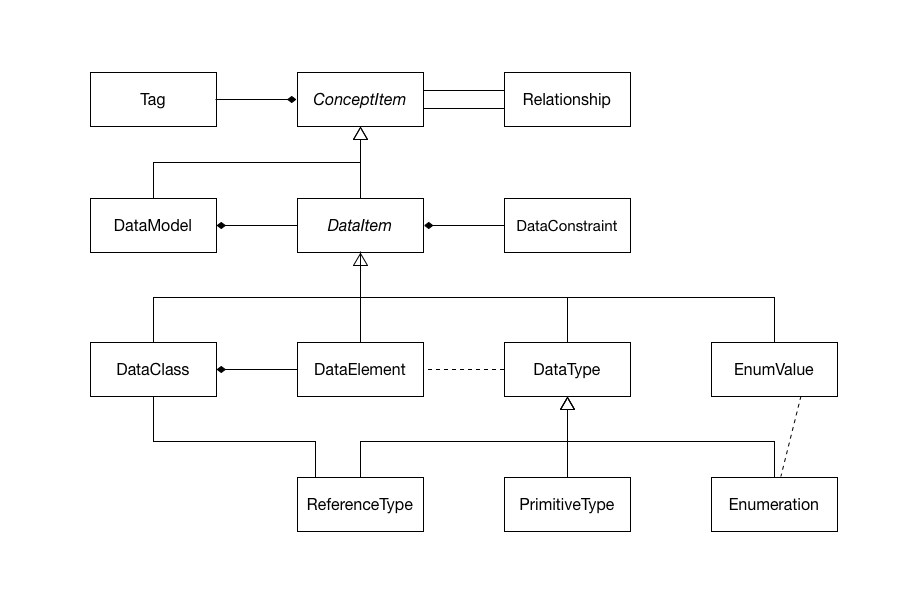
\includegraphics[width=1.0\textwidth,natwidth=610,natheight=642]{LemmaCore1}
\caption{Core Metamodel (Lemma)} 
\label{fig:lemma}
\end{figure}

Since all items are in effect \emph{ConceptItems} they can be considered to be representing a concept; furthermore all such items can have a relationship with any other conceptitem, and can be \emph{tagged} to reference items outside the registry, such as IRI's or webpages. Some of the core items in ISO11179-3 which are represented by UML diagrams can be directly represented in the core language, others are built in the manner described in the UML diagrams. 

The CaBIG registry was built on similar principles, but required a mapping algorithm to translate from UML to the ISO11179 Conceptual model as is documented in the paper by Kunz et al~\cite{Kunz2009}. In fact several mapping algorithms were tested, the main mapping is shown in Figure~\ref{fig:mapping}. By using a model based approach we avoid the need for such a mapping, instead our registry simply defines an ISO11179 view on the various datasets which are imported into the registry.  Some mapping algorithms are used in mapping XML to this model, and in comparing different dataitems within the registry.

\begin{figure}[h]
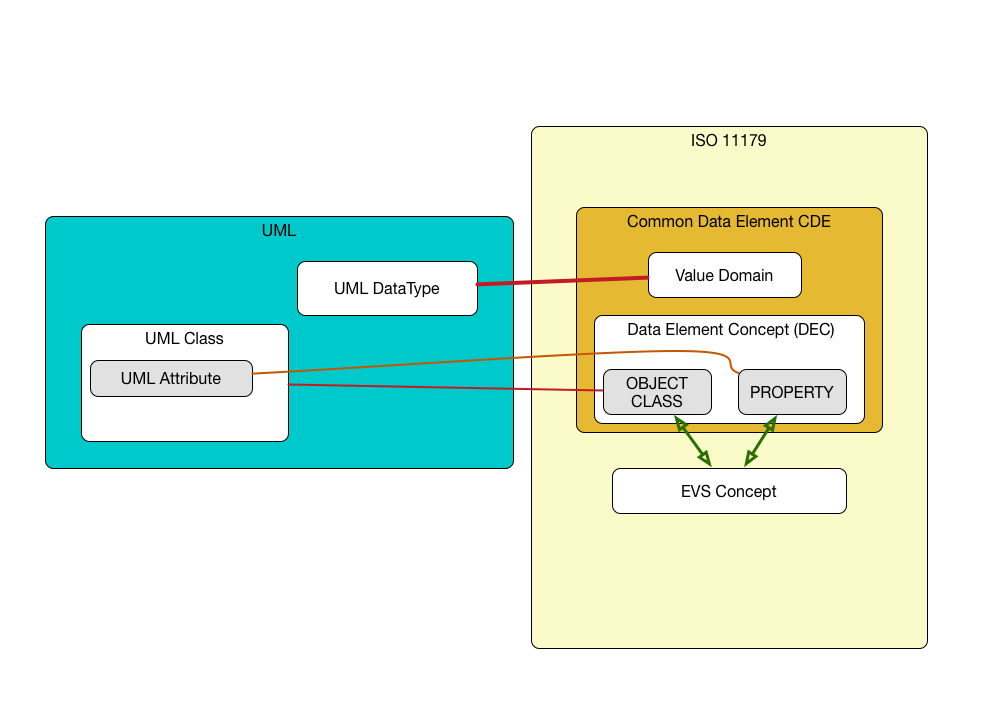
\includegraphics[width=1.0\textwidth,natwidth=610,natheight=642]{ISOUMLTransform}
\caption{CaBIG ISO to UML Tranform} 
\label{fig:mapping}
\end{figure}



\subsection{Registry Contents}



All of our conceptitems in the registry will have identifiers, unique within the context of the registry, this implements Rule 1 of the previous section.  Classes will be uniquely named within models, elements will be uniquely named within classes.  
\begin{zed}
  [Id, Name]
\end{zed}

A data element has multiplicity: the three values that are important
to us are as follows:
\begin{syntax}
  Multiplicity & ::= & \optional \mid \mandatory \mid \many 
\end{syntax}

It has also ordering 
\begin{syntax}
  Ordering & ::= & ordered \mid notOrdered 
\end{syntax}

Although a registry could support other kinds of link, there are two that are important to us here: $extends$ and $newVersionOf$. These refer to other items, using identifiers rather than names. The intended semantics of an conceptitem consists primarily in its textual explanation.  Additional information comes from any other items that contain the element: the class, and the model. We introduce the \emph{Interpretation}.
\begin{zed}
  [Interpretation]
\end{zed}
A piece of text can be interpreted in multiple ways, and thus: 
\begin{zed}
  Text == \power Interpretation
\end{zed}

The language is a language of \emph{metadata} and it will normally sit within the context of a metadata registry or similar server artefact. The core entity in our new model is the \emph{ConceptItem} which is in effect an abstract entity from which most of the other entity derive. At its core is the idea that it represents a concept in some shape or form, and that we can make the name and text description originate from a vocabulary or terminology server. As an entity it can be related to any other entity in the registry using the Relationship artefact. Versioning control is handled through the use of a GUID, which has the added benfit of turning metadata into \emph{linked metadata} automatically. The Tag class allows any vocabulary or ontology element to be associated with any registry item. This ensures the import of standard ontologies into a metadata registry built around this metamodel.

\begin{schema}{ConceptItem}
  id : Id \\
  name : Name \\
  text : Text \\
  kind : Kind \\  
  extends, newVersionOf : \power Id
\end{schema}

\subsubsection{DataModel}

 DataModel is a versioning and grouping mechanism for one metadata-set, it might for instance be metadata connected with a particular database, or a particular XSD Schema which is used in a particular domain, however it allows us to group and version a related set of DataClasses.  A DataModel can contain many DataElements, and many DataTypes. A DataModel contains one or more DataItems, which may be implemented as DataClasses, DataElements, DataTypes or EnumerationValues. As all DataItems are also ConceptItems, they can have Tags, which link them to entities outside that DataModel using URI's, and they can have Relationships which are two-way associations with other ConceptItems. DataConstraints are attached to each DataItem in the DataModel. A DataModel also declares a status, which can be draft or final.

\begin{syntax}
  Status & ::= & \draft \mid \final 
\end{syntax}

Each datamodel has a globally unique identifier.  
\begin{zed}
  [GUID]
\end{zed}

\begin{schema}{DataModel}
  ConceptItem \\
  guid : GUID \\
  dataclasses, dataelements, datatypes, enumerations, primitivetypes : \power Id \\
  imports : \power Id \\
  status : Status 
  \where
  kind = \datamodel
\end{schema}


\subsubsection{DataItem}
A DataItem is child artefact of a ConceptItem, with the ability to contain a DataConstraint. DataConstraints may be described in the context of any sub-type of a DataItem, that is DataElement, DataType, Enumeration or Enum. Since DataModels contain DataItems one can also group the conjunction of constraint information at the DataModel level.  All that we need to know of DataConstraints is that an implication ordering exists as a partial order upon this given type. 

\begin{zed}
  [DataConstraint]
\end{zed}

%%inrel \Cimplies 
\begin{axdef}
  \_ \Cimplies \_ : DataConstraint \rel DataConstraint 
  \where
  \id DataConstraint \subseteq (\_ \Cimplies \_) \\
  (\_ \Cimplies \_) \cap (\_ \Cimplies \_) \inv = \id DataConstraint   
\end{axdef}



\begin{schema}{DataItem}
 ConceptItem \\
 dataConstraint : DataConstraint \\
\end{schema}


\subsubsection{DataClass}
A DataClass is a mechanism for grouping DataItems, which are atomic pieces of data. A concept may be represented by a DataClass or a DataElement, but the DataItem is the atomic component of that DataClass, it can't be reduced into any smaller component. A DataClass can be used as a DataItem, in that it can be contained within another DataClass, and so it can be used to provide multi-level grouping within a DataModel. A DataClass can \emph{extend} another DataClass, this \emph{inheritance} mechanism is very straightforward since we are only considering structure and not behaviour; it allows the child class to have all the member DataItems and DataClasses that are present in the parent. These DataItems and DataClasses are in effect references, so that if the parent class changes then these \emph{inherited} DataItems and DataClasses will be changed as well.
For the formal specification of the DataClass, we record extension and composition relationships.

\begin{schema}{DataClass}
  DataItem \\
  dataelements : \power Id \\
  extends : \power Id \\
  components : \power Id 
  \where
  kind = \dataclass
\end{schema}

\subsubsection{DataElement}

A DataElement is the smallest data entity described in this langauge, it has a direct one to one relationship with a DataType, since every DataElement will have a corresponding DataType. DataElements have multiplicity and ordering. 

\begin{schema}{DataElement}
  DataItem \\
  multiplicity : Multiplicity \\
  ordering : Ordering \\
  dataType : Id 
  \where
  kind = \dataelement
\end{schema}

\subsubsection{DataTypes}

Enumerations have a sequence of references to values. 

\begin{schema}{Enumeration}
  DataItem \\
  enums : \power Id 
  \where
  kind = \enumeration
\end{schema}

Enumerated values have a value.  

\begin{zed}
  [Value]
\end{zed}

\begin{schema}{Enum}
  DataItem \\
  value : Value 
  \where
  kind = \enum 
\end{schema}

And primitives are primitives. 

\begin{schema}{PrimitiveType}
  DataItem \\
  values : \power Value 
  \where
  kind = \primitivetype
\end{schema}

\subsubsection{Items}

Here we are looking at any language entity which could be present in a registry, an item could be any of the following artefacts, all of which will be kept within a metadata registry.

\begin{zed}
  Item \defs DataModel \lor DataClass \lor DataElement \lor DataType \\
                                            \lor PrimitiveType  \lor Enumeration \lor Enum
\end{zed}

************ Need to include Tag, Relationship, ReferenceType



\subsection{The Registry Itself}

A registry is an indexed collection of items. 

The path to an item starts with the guid of a model, and is then followed by a sequence of names. 
\begin{zed}
  Path == \seq Name 
\end{zed}

\begin{schema}{Concept\_Items}
  item : Id \pfun Item \\
  items : \power Id \\
  path : Id \pfun Id \pfun Path 
\end{schema}

We introduce names for the sets of identifiers pointing to different
kinds of items:

\begin{schema}{Registry\_Sets}
  datamodels, dataclasses, dataelements, enumerations, datatypes, \\
  primitivetype, enums : \power
  Id 
\end{schema}

We introduce also the `global' relationships implied by the reference-valued attributes $extends$ and $newVersionOf$:

%%inrel \refines \newVersionOf
\begin{schema}{Registry\_Links}
  \_ \extends \_, \_ \newVersionOf \_ : Id \rel Id 
\end{schema}

Similarly, we introduce the global relationships implied by containment: 

%%inrel \contains \extends
\begin{schema}{Registry\_Structure}
  \_ \contains \_ : Id \rel Id \\
  datamodel : Id \pfun Id \\
  contents, scope : Id \pfun \power Id \\
  values : Id \pfun \power Value 
\end{schema}

We may now describe registry properties in terms of the combination of all of these identifiers:

\begin{schema}{Registry\_Contents}
  Registry\_Items \\
  Registry\_Sets \\
  Registry\_Links \\
  Registry\_Structure
\end{schema}

\subsubsection{Consistency and derivation}


\begin{schema}{Registry\_Items\_Derivation}
  Registry\_Contents
  \where
  \dom conceptitem = conceptitem \\
  \forall m : datamodels ; i : conceptitems \spot {} \\ \t1 
  \LET c == (\mu x : dataclasses \mid i \in (conceptitem~x).elements) \spot
  {} 
  \\ \t2 
  path~m~i = \langle (conceptitem~m).name, (conceptitem~c).name, (conceptitem~i).name
  \rangle 
\end{schema}

\begin{schema}{Registry\_Sets\_Derivation}
  Registry\_Contents
  \where 
  datamodels = \{ i : \dom conceptitem \mid (conceptitem~i).kind = \datamodel \} \\
  dataclasses = \{ i : \dom conceptitem \mid (conceptitem~i).kind = \dataclass \} \\
  dataelements = \{ i : \dom conceptitem \mid (conceptitem~i).kind = \dataelement \} \\
  enumerations = \{ i : \dom conceptitem \mid (item~i).kind = \enumeration \} \\
  primitivetypes = \{ i : \dom conceptitem \mid (conceptitem~i).kind = \primitivetype \} \\
  enums = \{ i : \dom conceptitem \mid (conceptitem~i).kind = \enum \} \\
  \dom conceptitem = \bigcup \{ datamodels, dataclasses, dataelements, enumerations,
  primitivetypes, enums \} \\
  final = \bigcup \{~i : datamodels \mid (conceptitem~i).status = \final \spot \{ i \}
  \cup contents~i~\} 
\end{schema}

\begin{schema}{Registry\_Links\_Derivation}
  Registry\_Contents 
  \where 
  (\_ \newVersionOf \_) \in datamodels \rel datamodels \\
  (\_ \refines \_) \in {} \\ \t1 
  (dataclasses \rel classes) \cup (dataelements \rel
  dataelements) \cup (enums \rel enums) \\
  \forall i,j : \dom conceptitem \spot {} \\
  \t1 i \newVersionOf j \iff j \in (conceptitem~i).newVersionOf \land {} \\
  \t1 i \extends j \iff j \in (conceptitem~i).extends 
\end{schema}

That is, only models are versioned, and every semantic link connects two items of the same kind, whether these are dataclasses, dataelements, or values.

One item is contained within another if it is declared and managed in the context of that other item: for example, every element is declared in the context of a unique dataclass, and every item is declared in the context of a datamodel.  For convenience, we define not only a $contains$ relation, between references, but also a $contents$ function, returning references to all of the items contained within a referenced item.

The $extends$ function is more straightforward. 

\begin{schema}{Registry\_Structure\_Derivation\_Contents}
  Registry\_Contents
  \where
  \forall m : datamodels \spot contents~m = {} \\
  \t1 (item~m).dataclasses \cup (item~m).enumerations \cup
  (item~m).primitivetypes \cup {} \\
  \t1 \bigcup \{~c : (item~m).dataclasses \spot contents~c~\} \cup {} \\
  \t1 \bigcup \{~n : (item~m).enumerations \spot contents~n~\}
  \\
  \forall c : dataclasses \spot contents~c = {} \\
  \t1 (item~c).dataelements  \cup {} \\
  \t1 \bigcup \{~s : (item~c).components \spot contents~s ~\}
  \\
  \forall n : enumerations \spot contents~n = (item~n).enums
  \\
  \dom contents = \bigcup \{ datamodels,data classes, enumerations \} 
  \\
  \bigcup (\ran contents) = \bigcup \{ dataclasses, dataelements, enumerations, enums,
  primitivetypes \} 
  \\
  \forall i : \dom item \spot contents~i = (\_ \contains \_) ~\limg \{ i \}
  \rimg \\
  (\_ \extends \_) \in dataclasses \rel dataclasses \\
  \forall c, d : dataclasses \spot c \extends d \iff 
  d \in (item~c).extends
\end{schema}

That is, the contents of a model includes the contents of any classes and enumerations that it contains, a class contains its elements, and an enumeration contains its values.  Only models, classes, and enumerations have contents, and only classes, elements, enumerations, values, and primitives---not models---can be contained. 

A related but not equivalent notion is that of the `scope' of a model. This is a set of references to every item contained within that model, or contained within a model that it `imports'. 

\begin{schema}{Registry\_Structure\_Derivation\_Scope}
  Registry\_Contents
  \where
  \dom scope = datamodels 
  \\
  \forall m : datamodels \spot scope~m = contents~m \cup \bigcup 
  ( contents~ \limg (item~m).imports \rimg )
\end{schema}

It will be convenient also to consider the inverse relational image of the closure of this function.  For any non-model item in the registry, this will return a reference to the unique datamodel containing that item. 

\begin{schema}{Registry\_Structure\_Derivation\_Model}
  Registry\_Contents
  \where
  \dom model = \bigcup \{ dataclasses, dataelements, enumerations, enums,
  primitivetypes \} \\
  datamodel = ((\_ \contains \_)\star)\inv \rres datamodels
\end{schema}

\begin{zed}
  Registry\_Structure\_Derivation \defs {} \\ \t1 
  Registry\_Structure\_Derivation\_Contents \land {} \\ \t1 
  Registry\_Structure\_Derivation\_Scope \land {} \\ \t1 
  Registry\_Structure\_Derivation\_Model   
\end{zed}

\begin{zed}
  Registry\_Derivation \defs {} \\ \t1 
  Registry\_Sets\_Derivation \land {} \\ \t1 
  Registry\_Links\_Derivation \land {} \\ \t1 
  Registry\_Structure\_Derivation 
\end{zed}

\subsection{Registry Properties}

A datamodel can import only other datamodels known to the registry.

\begin{schema}{Registry\_Imports}
  Registry\_Contents 
  \where
  \forall m : datamodels \spot (item~m).imports \subseteq datamodels
\end{schema}

Every reference to a type must be to a type known to the registry: a known dataclass, enumeration, or primitivetype. 

\begin{schema}{Registry\_TypesDefined}
  Registry\_Contents
  \where
  \forall e : dataelements \spot (item~e).type \in dataclasses \cup enumerations \cup
  primitives 
\end{schema}

A datamodel may be a new version only of a finalised datamodel.  A datamodel may be final only if all imported datamodel are also final.  An item may be finalised only if all of its outgoing semantic links are to finalised items.

\begin{schema}{Registry\_Final}
 Registry\_Contents
  \where
  \ran (\_ \newVersionOf \_) \subseteq final \\
  \forall f : final \cap datamodels \spot (item~f).imports \subseteq final \\
  (\_ \refines \_) \limg final \rimg \subseteq final 
\end{schema}

\begin{zed}
  Registry\_Properties \defs {} \\ \t1
  Registry\_Imports \land {} \\ \t1 
  Registry\_TypesDefined \land {} \\ \t1
  Registry\_Final 
\end{zed}

\subsection{Semantics}

***************NEEDS REVISION*************************

The `semantics' of a data element is a mapping from possible values to \emph{a set of} possible interpretations.  Or, equally, a \emph{relation} between values and interpretations. 

The intended interpretation of a given value, in the context of a given registry, will depend upon:
\begin{itemize}
\item the text describing the value
\item the text describing the value type (primitive, enumerated or referenced)
\item the text describing the dataelement
\item the text describing the dataclass in which the element is defined,
  and any dataclasses `containing' that dataclass
\item the text describing the datamodel containing the dataelement
\item the text of any item that these items are linked to using$\extends$ 
\end{itemize}
Any of this text---even that which has been attached to a primitive value domain---may have something specific to say about a given data element.  


\section{Metadata Management}
This section gives a brief overview of the tasks which data registration authorities face, the principle problem being what data is held where, what formats are being used and how does it relate to other datasets being managed directly or indirectly. It could be that one data item has a reference to another data item managed by a different authority and the only reference is a written instruction stating that this \emph{dataitem is not the same as that dataitem}. 

The principal tasks faced by a data registration authority are given as:
\begin{itemize}
\item Creation of new datasets
\item Curation of existing datasets
\item Merging of existing datasets
\item Querying over existing datasets
\end{itemize}

The first task or use case is relatively straightforward, however there is one aspect that needs discussion. Very often datasets are developed by teams, and often using tools that are not really designed for dataset development. In the NHS we have found that many datasets are initially developed by domain experts using Excel, mostly because it is accessible and is easy to interpret at a high level. One of the biggest problems encountered here is simply co-ordination amongst the contributors. 

The next task is curation of existing datasets, once a dataset is published and is being used it's shortcomings will be noted by users who will lobby for changes. Datasets are easier to manage if they conform to the Open-Closed Principle of software engineering, first introduced by Bertram Meyer \cite{Meyer} which states that a module should be open to extension and closed to change. This means that datasets or datamodels can be extended by being added to, but that existing items should not be changed. Changing is possible, but it implies the start of a completely new DataModel, since it is very difficult to migrate existing artefacts from DataModel A to DataModel B if something has been removed or changed in A, however the addition of say another DataElement won't break existing artefacts.

The merging of datasets is another area of curation which is carried out by any registration authority and which is help by a metadata registry. The important points to note here are 1) the abiltiy to identify a particular element 2) the ability to relate it to another particular element and 3) the ability to measure the difference and decide which parts go into the merged dataset. Inevitably the mered dataset will contain back references to the originating dataitems, how easy these are to access and address is another point of note for the data curator.

The last point is the querying of data itself, although this is not really a function of a metadata registry, data querying is dependent on having data indexed in a structured manner, even if the data itself is stored in an unstructured manner. The better the index the better the search, and in many cases indexed searches on unstructured data can be fast and more effective that searches on data stored in normalized relational databases. 



\section{Results}

\subsection{Dataset Creation}





\subsection{Dataset Curation}





\subsection{Merging, linking and querying of Datasets}



\section{Discussion}

\section{Related Work}

 


\newpage

\bibliographystyle{plain}

\bibliography{md11179}

\end{document}

